\section{Технологический раздел}

В данном разделе будет проведен выбор средств реализации базы данных и приложения к базе данных.
Будут приведены описания реализаций сущностей базы данных, ограничений целостности и ролевой модели на уровне базы данных.
Будет приведена схема реализованного триггера, продемонстрирована его работоспособность и описан интерфейс для доступа к базе данных.

\subsection{Выбор средств реализации}

В подразделах ниже будет проведен выбор средств для реализации базы данных и приложения к базе данных.

\subsection*{Выбор СУБД}

Для реализации проектируемой базы данных подойдет любая реляционная СУБД с поддержкой ролевой модели.
В настоящей работе была выбрана PostgreSQL~\cite{psql} по следующим причинам:
\begin{itemize}
    \item открытый исходный код;
    \item поддержка полнотекстового поиска~\cite{psql};
    \item имеется опыт работы с данной СУБД.
\end{itemize}

\subsection*{Выбор языка программирования}

Для реализации приложения к проектируемое БД был выбран язык программирования Go~\cite{go} по следующим причинам:
\begin{itemize}
    \item простой синтаксис;
    \item быстрая компиляция~\cite{go};
    \item имеется стандартная библиотека для работы с SQL базами данных~\cite{gosql}.
\end{itemize}

\subsection*{Выбор среды разработки}

В качестве среды разработки был выбран Neovim~\cite{nvim} по следующим причинам:
\begin{itemize}
    \item данный текстовый редактор позволяет редактировать файлы с исходным кодом программы;
    \item быстрая и удобная навигация по файлам проекта;
    \item есть опыт использования данного текстового редактора.
\end{itemize}

\subsection{Описание реализаций}

В подразделах ниже будет приведено описание реализаций сущностей базы данных, ограничений целостности базы данных, ролевой модели на уровне базы данных и реализованного триггера для корректировки уровня доверия пользователей.

\subsubsection{Сущности базы данных}

В листингах \ref{lst:table:user} -- \ref{lst:table:token} приведены реализованные сущности базы данных.

\begin{code}
    \begin{lstinputlisting}[
            label={lst:table:user},
            caption={Создание User},
            firstline=2,
            lastline=10,
        ]{../src/sql/create_tables.sql}
    \end{lstinputlisting}
\end{code}

\begin{code}
    \begin{lstinputlisting}[
            caption={Создание Document},
            firstline=13,
            lastline=21,
        ]{../src/sql/create_tables.sql}
    \end{lstinputlisting}
\end{code}

\begin{code}
    \begin{lstinputlisting}[
            caption={Создание DocumentAuthor},
            firstline=24,
            lastline=27,
        ]{../src/sql/create_tables.sql}
    \end{lstinputlisting}
\end{code}

\begin{code}
    \begin{lstinputlisting}[
            caption={Создание Author},
            firstline=30,
            lastline=37,
        ]{../src/sql/create_tables.sql}
    \end{lstinputlisting}
\end{code}

\begin{code}
    \begin{lstinputlisting}[
            caption={Создание AnnotationTask},
            firstline=40,
            lastline=48,
        ]{../src/sql/create_tables.sql}
    \end{lstinputlisting}
\end{code}

\begin{code}
    \begin{lstinputlisting}[
            caption={Создание StructAnnotation},
            firstline=51,
            lastline=59,
        ]{../src/sql/create_tables.sql}
    \end{lstinputlisting}
\end{code}

\begin{code}
    \begin{lstinputlisting}[
            caption={Создание TermAnnotation},
            firstline=62,
            lastline=69,
        ]{../src/sql/create_tables.sql}
    \end{lstinputlisting}
\end{code}

\begin{code}
    \begin{lstinputlisting}[
            caption={Создание TermAnnotationPart},
            firstline=72,
            lastline=81,
        ]{../src/sql/create_tables.sql}
    \end{lstinputlisting}
\end{code}

\begin{code}
    \begin{lstinputlisting}[
            caption={Создание Sentence},
            firstline=84,
            lastline=88,
        ]{../src/sql/create_tables.sql}
    \end{lstinputlisting}
\end{code}

\begin{code}
    \begin{lstinputlisting}[
            label={lst:table:token},
            caption={Создание Token},
            firstline=91,
            lastline=96,
        ]{../src/sql/create_tables.sql}
    \end{lstinputlisting}
\end{code}

\newpage

\subsubsection{Ограничения целостности базы данных}

В листингах \ref{lst:cons:user} -- \ref{lst:cons:token} приведены реализованные ограничения целостности базы данных.

\begin{code}
    \begin{lstinputlisting}[
            label={lst:cons:user},
            caption={Ограничения User},
            firstline=1,
            lastline=13,
        ]{../src/sql/alter_tables.sql}
    \end{lstinputlisting}
\end{code}

\begin{code}
    \begin{lstinputlisting}[
            caption={Ограничения Document},
            firstline=15,
            lastline=29,
        ]{../src/sql/alter_tables.sql}
    \end{lstinputlisting}
\end{code}

\begin{code}
    \begin{lstinputlisting}[
            caption={Ограничения DocumentAuthor},
            firstline=37,
            lastline=46,
        ]{../src/sql/alter_tables.sql}
    \end{lstinputlisting}
\end{code}

\begin{code}
    \begin{lstinputlisting}[
            caption={Ограничения Author},
            firstline=31,
            lastline=35,
        ]{../src/sql/alter_tables.sql}
    \end{lstinputlisting}
\end{code}

\begin{code}
    \begin{lstinputlisting}[
            caption={Ограничения AnnotationTask},
            firstline=48,
            lastline=64,
        ]{../src/sql/alter_tables.sql}
    \end{lstinputlisting}
\end{code}

\begin{code}
    \begin{lstinputlisting}[
            caption={Ограничения StructAnnotation},
            firstline=66,
            lastline=83,
        ]{../src/sql/alter_tables.sql}
    \end{lstinputlisting}
\end{code}

\begin{code}
    \begin{lstinputlisting}[
            caption={Ограничения TermAnnotation},
            firstline=85,
            lastline=103,
        ]{../src/sql/alter_tables.sql}
    \end{lstinputlisting}
\end{code}

\begin{code}
    \begin{lstinputlisting}[
            caption={Ограничения TermAnnotationPart},
            firstline=105,
            lastline=117,
        ]{../src/sql/alter_tables.sql}
    \end{lstinputlisting}
\end{code}

\begin{code}
    \begin{lstinputlisting}[
            caption={Ограничения Sentence},
            firstline=119,
            lastline=125,
        ]{../src/sql/alter_tables.sql}
    \end{lstinputlisting}
\end{code}

\begin{code}
    \begin{lstinputlisting}[
            label={lst:cons:token},
            caption={Ограничения Token},
            firstline=127,
            lastline=133,
        ]{../src/sql/alter_tables.sql}
    \end{lstinputlisting}
\end{code}

\newpage

\subsubsection{Ролевая модель на уровне базы данных}

В листинге \ref{lst:roles} приведена реализованная ролевая модель на уровне базы данных.

\begin{code}
    \begin{lstinputlisting}[
            label={lst:roles},
            caption={Создание ролей и пользователей},
            firstline=1,
            lastline=25,
        ]{../src/sql/create_roles.sql}
    \end{lstinputlisting}
\end{code}

\newpage

\subsubsection{Функции, процедуры и триггеры}

На рисунке \ref{fig:trig-impl} представлена реализация функции триггера, отвечающего за пересчет уровня доверия пользователей.

\begin{figure}[H]
	\centering
	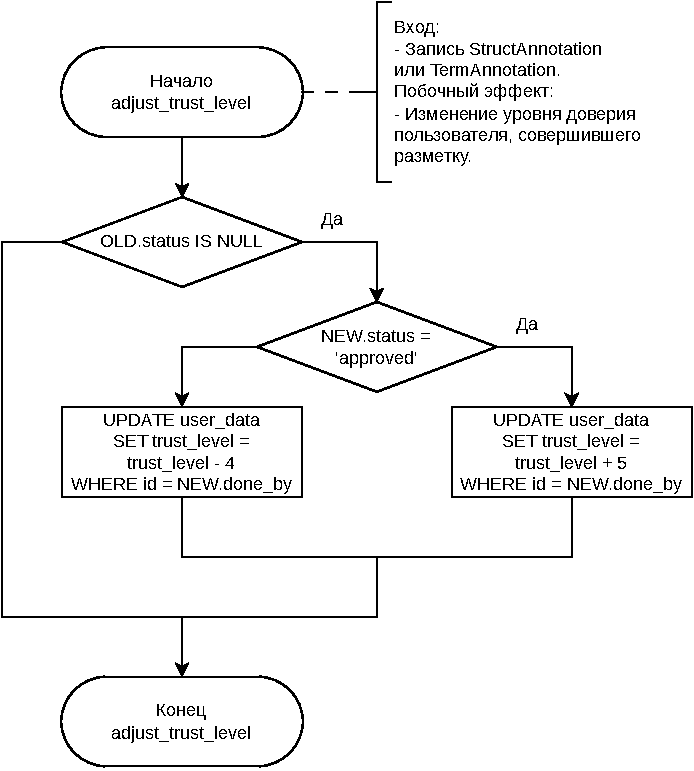
\includegraphics[width=0.7\textwidth]{diag/tech-trig-v4.pdf}
	\caption{Схема реализации алгоритма работы триггера, отвечающего за пересчет уровня доверия пользователей на языке plpgsql}
	\label{fig:trig-impl}
\end{figure}

\subsection{Тестирование функций}

% Описание методов тестирования и тестовых кейсов для всех разработанных на стороне базы данных функций;

В листингах \ref{lst:test:trig:approved}, \ref{lst:test:trig:rejected} продемонстрирована работоспособность реализованного триггера.

\begin{code}
    \begin{lstinputlisting}[
            label={lst:test:trig:approved},
            caption={Увеличение уровня доверия пользователя при одобрении его разметки},
        ]{lst/trig-approved.sql}
    \end{lstinputlisting}
\end{code}

\begin{code}
    \begin{lstinputlisting}[
            label={lst:test:trig:rejected},
            caption={Уменьшение уровня доверия пользователя при отклонении его разметки},
        ]{lst/trig-rejected.sql}
    \end{lstinputlisting}
\end{code}

\subsection{Интерфейс доступа к базе данных}

В таблице ниже представлен интерфейс доступа к базе данных, осуществляемого с помощью REST API~\cite{restapi}.
% XXX не полный и не полностью реализованный, но об этом знать не обязательно

\begin{table}[H]
\centering
\caption{Интерфейс доступа к базе данных}
\begin{tabular}{|m{2cm}|m{2.5cm}|m{10.5cm}|}
\hline
    \textbf{Метод} & \textbf{URL} & \textbf{Описание} \\ \hline
    % GET & /register & Получение страницы для регистрации \\ \hline
    POST & /register & Регистрация пользователя с введенными именем пользователя, адресом почты и паролем \\ \hline
    % GET & /login & Получение страницы для входа в систему \\ \hline
    POST & /login & Вход в систему по имени пользователя и паролю \\ \hline
    % GET & /profile & Получение личной страницы пользователя \\ \hline
    GET & /d/\{id\} & Получение текста документа с указанным id \\ \hline
    POST & /d & Добавление нового документа \\ \hline
    GET & /tasks & Получение списка заданий для разметки \\ \hline
    GET & /task/\{id\} & Получение страницы с конкретной задачей на разметку \\ \hline
    POST & /task & Создание нового задания на разметку \\ \hline
    GET & /annot/\{id\} & Получение разметки с указанным id \\ \hline
    POST & /annot & Добавление новой разметки \\ \hline
    GET & /search & Получение страницы для поиска по корпусу \\ \hline
    POST & /search & Выполнение поиска по корпусу \\ \hline
\end{tabular}
\label{tab:api}
\end{table}

% \newpage

\subsection*{Вывод}

В данном разделе был проведен выбор средств реализации базы данных и приложения к базе данных.
Были приведены описания реализаций сущностей базы данных, ограничений целостности и ролевой модели на уровне базы данных.
Была приведена схема реализованного триггера, продемонстрирована его работоспособность и описан интерфейс для доступа к базе данных.
